%%%%%%%%%%%%%%%%%%%%%%%%%%%%%%%%%%%%%%%%%%%%%%%%%%%%%%%%%%%%%%%%%%
%%%%%%%%%%%%%%%%%%%%%%%%%%%%%%%%%%%%%%%%%%%%%%%%%%%%%%%%%%%%%%%%%%
%Packages
\documentclass[11pt, a4paper]{article}
\usepackage{geometry}
\geometry{margin=1in}
\usepackage{setspace}
\singlespacing
\usepackage[top=3cm, bottom=4cm, left=3.5cm, right=3.5cm]{geometry}
\usepackage{amsmath,amsthm,amsfonts,amssymb,amscd, fancyhdr, color, comment, graphicx, environ}
\usepackage{float}
\usepackage{parskip}
\usepackage{mathrsfs}
\usepackage[math-style=ISO]{unicode-math}
\usepackage{lastpage}
\usepackage[dvipsnames]{xcolor}
\usepackage[framemethod=TikZ]{mdframed}
\usepackage{enumerate}
\usepackage[shortlabels]{enumitem}
\usepackage{fancyhdr}
\usepackage{indentfirst}
\usepackage{listings}
\usepackage{sectsty}
\usepackage{thmtools}
\usepackage{shadethm}
\usepackage{hyperref}
\usepackage{setspace}
\usepackage{amsmath}
\usepackage[backend=biber, style=authoryear]{biblatex}

\hypersetup{
    colorlinks=true,
    linkcolor=blue,
    filecolor=magenta,      
    urlcolor=blue,
}
%%%%%%%%%%%%%%%%%%%%%%%%%%%%%%%%%%%%%%%%%%%%%%%%%%%%%%%%%%%%%%%%%%
%%%%%%%%%%%%%%%%%%%%%%%%%%%%%%%%%%%%%%%%%%%%%%%%%%%%%%%%%%%%%%%%%%
%Environment setup
\mdfsetup{skipabove=\topskip,skipbelow=\topskip}
\newrobustcmd\ExampleText{%
An \textit{inhomogeneous linear} differential equation has the form
\begin{align}
L[v ] = f,
\end{align}
where $L$ is a linear differential operator, $v$ is the dependent
variable, and $f$ is a given non−zero function of the independent
variables alone.
}
\mdfdefinestyle{theoremstyle}{%
linecolor=black,linewidth=1pt,%
frametitlerule=true,%
frametitlebackgroundcolor=gray!20,
innertopmargin=\topskip,
}
\mdtheorem[style=theoremstyle]{Problem}{Problem}
\newenvironment{Solution}{\textbf{Solution.}}

\definecolor{codegreen}{rgb}{0,0.6,0}
\definecolor{codegray}{rgb}{0.5,0.5,0.5}
\definecolor{codepurple}{rgb}{0.58,0,0.82}
\definecolor{backcolour}{rgb}{0.95,0.95,0.92}

\lstdefinestyle{mystyle}{
    backgroundcolor=\color{backcolour},   
    commentstyle=\color{codegreen},
    keywordstyle=\color{magenta},
    numberstyle=\tiny\color{codegray},
    stringstyle=\color{codepurple},
    basicstyle=\ttfamily\footnotesize,
    breakatwhitespace=false,         
    breaklines=true,                 
    captionpos=b,                    
    keepspaces=true,                 
    numbers=left,                    
    numbersep=5pt,                  
    showspaces=false,                
    showstringspaces=false,
    showtabs=false,                  
    tabsize=2
}

\lstset{style=mystyle}
%%%%%%%%%%%%%%%%%%%%%%%%%%%%%%%%%%%%%%%%%%%%%%%%%%%%%%%%%%%%%%%%%%
%%%%%%%%%%%%%%%%%%%%%%%%%%%%%%%%%%%%%%%%%%%%%%%%%%%%%%%%%%%%%%%%%%
%Fill in the appropriate information below
\newcommand{\norm}[1]{\left\lVert#1\right\rVert}     
\newcommand\course{XXXX0000}                            % <-- course name   
\newcommand\hwnumber{0}                                 % <-- homework number
                     % <-- personal information
%%%%%%%%%%%%%%%%%%%%%%%%%%%%%%%%%%%%%%%%%%%%%%%%%%%%%%%%%%%%%%%%%%
%%%%%%%%%%%%%%%%%%%%%%%%%%%%%%%%%%%%%%%%%%%%%%%%%%%%%%%%%%%%%%%%%%
%Page setup
\pagestyle{fancy}
\headheight 35pt
\lhead{\today}
\rhead{
\includegraphics[width=2.5cm]{bse_logo.png}}
\lfoot{}
\pagenumbering{arabic}
\cfoot{\small\thepage}
\rfoot{}
\headsep 1.2em
\renewcommand{\baselinestretch}{1.25}
%%%%%%%%%%%%%%%%%%%%%%%%%%%%%%%%%%%%%%%%%%%%%%%%%%%%%%%%%%%%%%%%%%
%%%%%%%%%%%%%%%%%%%%%%%%%%%%%%%%%%%%%%%%%%%%%%%%%%%%%%%%%%%%%%%%%%
%Add new commands here
\renewcommand{\labelenumi}{\alph{enumi})}
\newcommand{\Z}{\mathbb Z}
\newcommand{\R}{\mathbb R}
\newcommand{\Q}{\mathbb Q}
\newcommand{\NN}{\mathbb N}
\newcommand{\PP}{\mathbb P}
\DeclareMathOperator{\Mod}{Mod} 
\renewcommand\lstlistingname{Algorithm}
\renewcommand\lstlistlistingname{Algorithms}
\def\lstlistingautorefname{Alg.}
\newtheorem*{theorem}{Theorem}
\newtheorem*{lemma}{Lemma}
\newtheorem{case}{Case}
\newcommand{\assign}{:=}
\newcommand{\infixiff}{\text{ iff }}
\newcommand{\nobracket}{}
\newcommand{\backassign}{=:}
\newcommand{\tmmathbf}[1]{\ensuremath{\boldsymbol{#1}}}
\newcommand{\tmop}[1]{\ensuremath{\operatorname{#1}}}
\newcommand{\tmtextbf}[1]{\text{{\bfseries{#1}}}}
\newcommand{\tmtextit}[1]{\text{{\itshape{#1}}}}

\newenvironment{itemizedot}{\begin{itemize} \renewcommand{\labelitemi}{$\bullet$}\renewcommand{\labelitemii}{$\bullet$}\renewcommand{\labelitemiii}{$\bullet$}\renewcommand{\labelitemiv}{$\bullet$}}{\end{itemize}}
\catcode`\<=\active \def<{
\fontencoding{T1}\selectfont\symbol{60}\fontencoding{\encodingdefault}}
\catcode`\>=\active \def>{
\fontencoding{T1}\selectfont\symbol{62}\fontencoding{\encodingdefault}}
\catcode`\<=\active \def<{
\fontencoding{T1}\selectfont\symbol{60}\fontencoding{\encodingdefault}}
\addbibresource{references.bib} % the filename of your .bib file

%%%%%%%%%%%%%%%%%%%%%%%%%%%%%%%%%%%%%%%%%%%%%%%%%%%%%%%%%%%%%%%%%%
%%%%%%%%%%%%%%%%%%%%%%%%%%%%%%%%%%%%%%%%%%%%%%%%%%%%%%%%%%%%%%%%%%
%Begin now!



\begin{document}

\begin{titlepage}
    \begin{center}
        \vspace*{3cm}
            
        \Huge
        \textbf{Capstone Project:}
        \textbf{El Crim de la Guàrdia Urbana}
            
        \vspace{1cm}
        \huge
        Economics for Data Driven Decision Making
            
        \vspace{1.5cm}
        \Large
            
        \text{Guillem Mirabent Rubinat, Pere Pericot Masdevall}                      % <-- author
        
            
        \vfill
        \begin{center}21DM001 taught by Esther Hauk and Laurence Go \end{center}
        
        \vspace{1cm}
            
        
\includegraphics[width=0.4\textwidth]{bse_logo.png}
        \\
        
        \Large
        
        \today
            
    \end{center}
\end{titlepage}



%%%%%%%%%%%%%%%%%%%%%%%%%%%%%%%%%%%%%%%%%%%%%%%%%%%%%%%%%%%%%%%%%%
%%%%%%%%%%%%%%%%%%%%%%%%%%%%%%%%%%%%%%%%%%%%%%%%%%%%%%%%%%%%%%%%%%
%Start the assignment now
%%%%%%%%%%%%%%%%%%%%%%%%%%%%%%%%%%%%%%%%%%%%%%%%%%%%%%%%%%%%%%%%%%
%New problem
\newpage

\section*{I - Introduction}

Our intention is to model criminal cooperation in the face of a police investigation/interrogation. The departing point is very similar to that of the Prisoner’s Dilemma (from now on, PD) but extending the model in order to try to capture more complex behaviours as well. 

The model will be exemplified firstly using the case “El Crim de la Guàrdia Urbana” (from now on, CGU), to see how the development of the police investigation can affect the cooperation level of the criminals involved (based on the facts considered as proven by the final jury of this case in real life). The case is a great example to develop the model when there are only two players, which is what we aim to tackle in this project. Additionally, there are other factors that did not apply in the case of study or in general in the prisons of the EU, but that can be relevant in other parts of the world (or in the past here as well). Specifically, a factor to be taken into account is the concept  of becoming a “whistle-blower” which can, in the worst cases, mean the death of the “snitch” inside of the prison (or afterwards). Therefore, this can be a factor that needs to be taken into account when modelling criminal cooperation. What is very interesting about the CGU is that the strategies that both players chose changed as new evidence was found by the police. Therefore, it will be a very good example to showcase how the game is modified as new information is revealed. 

Another interesting aspect is that this case showcases a unique instance of a kind of PD, but the players did not choose exactly at the same time without information. They were able to interact for some time before the final decision had to be made and, therefore, we are able to see, through the case, how an initial effort to cooperate (even fuelled by their mutual love and life project together) could turn to a visceral exchange of accusations when the right incentives appeared (or, at least, when the players felt that those incentives had appeared due to their limited capacity to comprehend other alternatives). Our approach will be to analyse the real case scenario of the Iterated Prisoner’s Dilemma (from now on, IPD).  

The final aim of our model would be to be general enough that it could be applied to different situations and be used to explain criminal cooperation in a more specific way than the standard PD.

\section*{II - \textit{Statu Ars et Scientia}}

The PD has been extensively analysed by the academia. This analysis comes from not only Economists but also from Jurists and Criminologists (each from their own point of view, being Economists and Mathematicians the only valuable source of a Game Theory approach to it). The analysis published hitherto, though, approaches the PD as either a single game or a series of single games (IPD). We will, of course, use this same approach as a starting point but, coming from our specific case, we will also consider the possibility that the game, when encountered in real life, becomes a mixture of both. For this, we will consider the fact that usually there is no such thing as IPD regarding real life criminals (although the abstractions on cooperation decisions remain useful in other areas of life) nor is there a single game being played but rather criminals usually face a sort of mixed PD where they Iterate the game until some crucial point arrives and the state of the last game becomes the final state.   

That being said, we do enjoy the conclusions of some of the research that has been done hitherto, so we are going to mention the most important findings.

The single iteration of the PD is not as interesting in its basic form, but IPD does offer interesting possibilities. There has been a lot of interest around it and the conclusions are different every time depending on the specific constraints. Most of the findings come from competitions where participants provided models that were then faced against one another for many iterations of the PD. Once strategies like Grim-Trigger (which essentially converts the IPD into a sort of ultimatum game) or TitForTat appeared, the free-riders were swiftly eliminated and got very bad results. It seemed that some sort of cooperation with threatening or complex non-naïve cooperative systems were the solution. On other competitions, though, “simpler” strategies like OmegaTitForTat (which was slightly more complex than the basic version of just reacting in the next round with whatever the opponent did in the previous one), outperformed more complex systems of strategies. In competitions where participants were allowed to present more than one strategy bot, the groups that had enhanced cooperation with other members of the group outperformed other strategies. Among them, there were approaches where the participants in the group always cooperated among them while playing OmegaTitForTat or other simple strategies with the rest of the participants, or another very interesting approach called “La Cosa Nostra” which had a “Godfather” who always betrayed its cooperative “Hitmen” (so the group played to favour the Godfather, while the rest of the group always cooperated when against other members), which in their turn always played to inflict the most damage possible to non-members. This sort of strategies proved very effective, which shows that trust was an important element in obtaining good results in the competitions. Knowing that the other part would cooperate because it was from the same group allowed members to cooperate safely and, thus, obtain better results in the iterations where they faced other members. 

\section*{III - Models}

\subsection*{First Model: Basic game and criminal case description}


In this first version of the model, shown in Table 1, we have taken an approximation to how the output matrices would look like from a classical single iteration PD standpoint. It’s a very simplified model, of course, but at the same time it offers a simplified overview of the extreme outputs they were facing. All of the numbers are computed considering how the criminal legal system in Spain works and how high the sentences are in years for the crimes they committed. The facts that are used to compute these are, for simplicity’s sake, the official record from the case and, in general, what has come to be considered the “proven facts”, which are deemed as true beyond reasonable doubt.

\begin{table}[h]
\centering
\begin{tabular}{cc|c|c|}
\cline{3-4}
& & \multicolumn{2}{c|}{Rosa} \\ \cline{3-4}
& & Betray & Cooperate \\ \hline
\multicolumn{1}{|c|}{Albert} & Betray & -20, -25 & -3, -25 \\ \cline{2-4}
\multicolumn{1}{|c|}{} & Cooperate & -20, -3 & -5, -5 \\ \hline
\end{tabular}
\caption{Years of prison faced}
\label{your_label_here}
\end{table}

Albert: \[Y_{iBB} &= 20,  Y_{iBC} &= 3,  Y_{iCB} &= 20,  Y_{iCC} &\approx 5 \]

Rosa: \[Y_{jBB} &= 25,  Y_{jBC} &= 3,  Y_{jCB} &= 25,  Y_{jCC} &\approx 5 \]



The Case of the CGU has some very interesting legal complexities that, for obvious reasons, are not going to be covered. The simplified version of the case is that Albert López and Rosa Peral murdered Pedro Rodríguez jointly, with a plan that involved both of them. The three of them were police officers in the “Guàrdia Urbana de Barcelona” and were involved in a love triangle which had further complications. It was not just Albert versus Pedro for the love of Rosa, but there were added elements which finally tilted the opinion of the Tribunal to the joint murder version instead of just convicting Albert for it. 

In short as well, the versions for both Albert and Rosa were:

    • \textbf{Albert}: He argued that Rosa had a sort of “spell” on him and that he was so madly in love with her that when she called him saying that she had killed Pedro and needed him to help her burn his body, he just could not refuse. He said that he just was a silly guy who realized too late that Rosa was using him to cover her crime.

    • \textbf{Rosa}: She argued that Albert had threatened her and her daughters if she did not help him dispose of the cadaver. As a side note, as believable as this version could be a priori, it must be considered that the facts amounted to a point where it did not convince a tribunal composed by lay-people (lay as in “not versed in the Law”). It did not hold after a rigorous analysis by the police who investigated the crime\footnote{As a personal side note, the version did not hold due to problems started by Rosa herself. From a strictly Game Theory point of view, here general strategy could have been much better even while still choosing to betray Albert.}. 
    
Those versions are very relevant for a very simple reason, which is that both of them accepted some sort of participation in their own versions; they themselves accepted that they were, as a matter of fact, physically in the scene of the crime the night when it was committed, and also confessed to their participation in the crime (albeit in a limited manner, of course). This was crucial for the investigation as, prior to this “help”, the police was not yet able to prove their participation nor their location. They were not even capable of exactly determining the exact night of the crime until both suspects “kindly” decided to both coincide for the same moment in time in their own versions. After they started betraying each other, they were not able to deny their participation anymore, nor to play with location matters to deny being physically in the scene of the crime at the moment it was committed.

The numbers in the matrix represent years in prison as a result of the sentence. In the scenario where both Rosa and Albert betrayed each other, Rosa received a harsher sentence of 25 years due to an aggravating circumstance involving her partner. Albert, in contrast, received a sentence of 20 years. This disparity stemmed from Rosa's additional legal complication because Pedro was her fiancée, which increased her murder sentence.

When both chose cooperation, they would have received an expected prison time of 5 years each. However, due to the ambiguous nature of the evidence against them, the actual outcome could have varied widely – from minimal sentences to maximum penalties. Their collective job of leaving minimal traces complicated the case for the authorities, making it uncertain how the legal system would have treated them if they cooperated fully.

If one remained silent while the other betrayed, the maximum sentence for concealment under the Spanish Criminal Code would likely be 3 years. Yet, this could have been mitigated by extenuating circumstances, potentially reducing the sentence below 3 years. Importantly, their perception of the sentence differed significantly if only one of them was convicted, as they viewed the 20 or 25 years as an unjust penalty if the other was set free.

In our general case, we have that:

Two players: \(X_1, X_2\)

Two strategies: Betray (B), Cooperate (C)

Utilities: 
\[ u(X_{1B} | B), u(X_{1C} | C), u(X_{1B} | C), u(X_{1C} | B) \]
\[ u(X_{2B} | B), u(X_{2C} | C), u(X_{2B} | C), u(X_{2C} | B) \]

The conditions of identity for a PD game are, therefore:
\begin{align*}
u(X_{iC} | C) &> u(X_{iC} | B) &\text{ Where } i \text{ and } j \text{ are both players.} \\
u(X_{iB} | C) &> u(X_{iC} | C) \\
u(X_{iB} | B) &> u(X_{iC} | B)
\end{align*}

And finally, the condition for relevant results:
\begin{align*}
u(X_{iC} | C) &> u(X_{iB} | B)
\end{align*}

In our initial model, we have that $Y_{jBB} = Y_{jCB}$, and therefore in PD, there must be something else that makes $u(X_{iB} | B) > u(X_{iC} | B)$ true.

Therefore, we introduce $\Psi_i$ as the level of perceived injustice (assuming an egotistic sense of justice), having:

\begin{center}
$a \in \{ B_i, C_i \} \text{ and } b \in \{ B_j, C_j \}$,   
\end{center}


We now go from $u(X_{ia} | a) = -Y_{ab}$ to:
\begin{center}
\begin{equation}
    u(X_{ia} | a) = -\Psi_i - Y_{iab}
\end{equation} 
\text{for } \begin{cases} 
\Psi_i > 0, & \text{if } a = C \text{ and } b = B \\
0, & \text{otherwise} 
\end{cases}
\end{center}

The accurate determination of $\Psi_i$ would be a matter of high level psychological study which is not the object of this project. In our case, we are going to assume that $\Psi_i$ = 5, because it is a level that matches what both players receive if they cooperate.

Just to clarify, we assume that $\Psi_i > 0$ because it reflects the level of perceived injustice that anyone would feel if they got betrayed. Even if someone loves
someone else so much that they would not care, that would be the result of a different factor offsetting the effect of $\Psi_i$, and we are going to study this two
effects separately with $\Psi_i$ and $\Omega_i$.

As a matter of fact, the consideration of $\Psi_i$ is more a matter of completeness and rigorousity than practical relevance. Intuitively, this can be seen as the reason why being betrayed (C, B) is worse than both betraying (B, B). The conclusion is that this dilemma is just a matter of dialectics because the real issue with PD is choosing between both cooperating (C, C) or betraying the other (B, C). After this, if both players have incentives to betray, the conclusion is going to be (B, B) whether $\Psi_i$ = 0 or $\Psi_i$ > 0. If $\Psi_i$ > 0 their incentives to betray are going to be met quicker, but that is just a numeric movement.

The updated matrix, now converted to their perceived utility for the outputs, would look like:

\begin{table}[h]
\centering
\begin{tabular}{cc|c|c|}
\cline{3-4}
& & \multicolumn{2}{c|}{Rosa} \\ \cline{3-4}
& & Betray & Cooperate \\ \hline
\multicolumn{1}{|c|}{Albert} & Betray & -20, -25 & -3, -30 \\ \cline{2-4}
\multicolumn{1}{|c|}{} & Cooperate & -25, -3 & -5, -5 \\ \hline
\end{tabular}
\caption{Updated matrix using Equation 1 (with $\Psi_i = 5$)}
\label{your_label_here}
\end{table}

\subsection*{Second Model: Cooperation-promoting weights}

In order for players to cooperate, we know that $u(X_{iC} | C) > u(X_{iB} | C)$ must be met (cooperation condition).

If we assume that the Criminal Code is not greatly deficient and that $\Psi$ is only positive when an individual is "wronged", but not when the individual wrongs others (egotistic sense of injustice), then we would need additional elements to explain how the Nash Equilibrium (NE) can change to (C, C) instead of (B, B). In our case, the CGU, we initially got the element of love between the players (A, R). As we could define real love as incorporating the joint utility into one's own utility, we would effectively be in a case where:

\begin{center}
    \begin{equation}
        u(X_{ia} | b) = -\Psi_i - Y_{iab} - \Psi_j - Y_{jba}
    \end{equation}
\end{center}

In this case, however, we are considering a very specific case, in which the love is complete, real, effective and absolute. We could actually model all the possible levels of Love of individual i towards j ($L_i$), where $0 \leq L_i \leq 1$, as:

\begin{center}
    \begin{equation}
        u(X_{ia} | b) = -\Psi_i - Y_{iab} + L_i(-\Psi_j - Y_{jba})
    \end{equation}
\end{center}

We should even take into account the possibility that player i loves the other player so much that only their utility is taken into account; therefore (O)mega Love would be $\Omega_i$, where 0 $\leq \Omega_i \leq 1$:

\begin{center}
    \begin{equation}
        u(X_{ia} | b) = \Omega_i(-\Psi_i - Y_{iab}) + L_i(-\Psi_j - Y_{jba})
    \end{equation}
\end{center}

\textbf{Examples of how the model works:}

The basic PD game would be a case where $\Omega_i = 1$ and $L_i = 0$.

Given Equation 4, our matrix for the CGU if we assume players A and R really loved each other initially but not blindly ($\Omega_i = 1, L_i = 1$) would look like: 

\begin{table}[h]
\centering
\begin{tabular}{cc|c|c|}
\cline{3-4}
& & \multicolumn{2}{c|}{Rosa} \\ \cline{3-4}
& & Betray & Cooperate \\ \hline
\multicolumn{1}{|c|}{Albert} & Betray & -45, -45 & -33, -33 \\ \cline{2-4}
\multicolumn{1}{|c|}{} & Cooperate & -28, -28 & -10, -10 \\ \hline
\end{tabular}
\caption{CGU matrix given Equation 4 (Bonnie \& Clyde's matrix)}
\label{your_label_here}
\end{table}

As we can observe, now the NE is (C, C), as cooperating has become a strictly dominant strategy. Another interesting situation to analyze would be the matrix if Albert's version was true ($\Omega_A = 0, \Omega_R = 1, L_A = 1, L_R = 0$). If A is blindly in love with R but she is just using him, we would see that both players have the same utility levels, those of R:

\begin{table}[h]
\centering
\begin{tabular}{cc|c|c|}
\cline{3-4}
& & \multicolumn{2}{c|}{Rosa} \\ \cline{3-4}
& & Betray & Cooperate \\ \hline
\multicolumn{1}{|c|}{Albert} & Betray & -25, -25 & -30, -30 \\ \cline{2-4}
\multicolumn{1}{|c|}{} & Cooperate & -3, -3 & -5, -5 \\ \hline
\end{tabular}
\caption{CGU matrix given Equation 4 (A's Blind Lover matrix)}
\label{your_label_here}
\end{table}

In this case, as both players share R's utility levels, the NE is (C, B), as A "sacrifices" so that R can get her best utility level. The other version, which is based on fear, will be covered later.

As one final interesting scenario, we can analyze the selfless lovers, who have ($\Omega_A = 0, \Omega_R = 0, L_A = 1, L_R = 1$) and come, yet again, to the NE being (C, C):

\begin{table}[h]
\centering
\begin{tabular}{cc|c|c|}
\cline{3-4}
& & \multicolumn{2}{c|}{Rosa} \\ \cline{3-4}
& & Betray & Cooperate \\ \hline
\multicolumn{1}{|c|}{Albert} & Betray & -25, -20 & -30, -3 \\ \cline{2-4}
\multicolumn{1}{|c|}{} & Cooperate & -3, -25 & -5, -5 \\ \hline
\end{tabular}
\caption{CGU matrix given Equation 4 (Selfless Lovers' matrix)}
\label{your_label_here}
\end{table}

\subsubsection*{Cooperation condition at a specific point in time:}

We can now analyze at which levels of Love ($L_i$) and (O)mega Love ($\Omega_i$) the cooperation condition will hold:

\begin{center}
    $u(X_{iC} | C) > u(X_{iB} | C)$ 
\end{center}

\begin{center}
    $= \Omega_{i}(-\Psi_{i} - Y_{iCC}) + L_{i}(-\Psi_{j} - Y_{jCC}) > \Omega_{i}(-\Psi_{i} - Y_{iBC}) + L_{i}(-\Psi_{j} - Y_{jCB})$
    $= \Omega_{i}(0 - Y_{iCC} + 0 + Y_{iBC}) > L_{i}(-\Psi_{j} - Y_{jCB} + 0 + Y_{jCC})$
    \begin{equation}
        = \Omega_{i}(Y_{iBC} - Y_{iCC}) > L_{i}( Y_{jCC} - Y_{jCB} 
 - \Psi_{j})
    \end{equation}
\end{center}

We check the case for both i=A, j=R and i=R,j=A in our example, the CGU:

\textbf{\underline{i = A}}

$$
Y_{i B C}=3, \quad Y_{i C C}=Y_{j C C}=5, \quad y_{j C B}=25
$$
And assuming we used $\Psi_i=\Psi_j=5$:

$$
\Rightarrow \Omega_i(3-5)>L_i(5-25-5) \Rightarrow \Omega_i(-2)>L_i(-25)
$$
$$
\Rightarrow L_i > \frac{2 \Omega_i}{25} \quad \text{\textbf{(A's coop condition for the CGU case)}}
$$


As a matter of fact, for basic PD, $\Omega_i=1$ \&  $L_1=0$:

$2<0$ is false and thus the NE is (B,  B).

But as we have seen, for:
$$
\Omega_i=1 \, \& \, L_i=1 \rightarrow 2<25 \rightarrow N E \text { is }(C, C)
$$
$$
\Omega_A=0 \, \& \, L_A=1 \rightarrow 0<25 \rightarrow \text{Albert will cooperate}
$$ 

\textbf{\underline{i = R}}

$$
Y_{i B C}=3, \quad Y_{i C C}=Y_{j C C}=5, \quad Y_{j C B}=20
$$
And assuming we used $\psi_i=\psi_j=5$:
$$
\Rightarrow \Omega_i(3-5)>L_i(5-20-5)
$$
$$
\Rightarrow 2 \Omega_i<20 L_i \Rightarrow L_i > \frac{\Omega_i}{10} \quad 
\text{\textbf{(R's coop condition for the CGU case)}}
$$ 
In this case as well:
$$
\begin{aligned}
& \Omega_i=1 \, \& \, L_i=0 \rightarrow 1<0 \rightarrow N E \text { is }(B, B) \\
& \Omega_i=1 \, \& \, L_i=1 \rightarrow 1<10 \rightarrow N E \text { is }(C, C)
\end{aligned}
$$

Before looking at the model fit when taking Rosa's version into account, there is something to be pointed out. In Equation 4, we defined $L_i$ as the Love that player i felt towards the other player, and in the CGU case it is an appropriate assumption to take it as love. But there are many possible cooperation enhancing factors and the best thing about the model in (4) is that it is capable of capturing them all. Imagine a case where the players are not two lovers in the style of Bonnie and Clyde but rather a Godfather and a Hitman. The Hitman (H) might be weary of betraying the Godfather (G) and he might end up acting in the same way as the lovers did. Even further, he might be scared of not
favoring G's welfare and for that he might even act as a selfless lover (with $\Omega_i$ = 0 and $L_i$ = 1). As a result, then, we can conclude that the model we developed for the lovers case also works to represent every other possible mechanism used to enhance cooperation.

We can now actually discuss the matrix for Rosa's version, which is really just the opposite version of Albert's version matrix, but using fear as the cooperation catalyst instead of love. As Albert would be a more immediate threat, ($\Omega_A = 1, \Omega_R = 0, L_A = 0, L_R = 1$), giving as a result a NE on (B, C):

\begin{table}[h]
\centering
\begin{tabular}{cc|c|c|}
\cline{3-4}
& & \multicolumn{2}{c|}{Rosa} \\ \cline{3-4}
& & Betray & Cooperate \\ \hline
\multicolumn{1}{|c|}{Albert} & Betray & -20, -20 & -3, -3 \\ \cline{2-4}
\multicolumn{1}{|c|}{} & Cooperate & -25, -25 & -5, -5 \\ \hline
\end{tabular}
\caption{CGU matrix given Equation 4 (R's Coerced Cooperation matrix)}
\label{your_label_here}
\end{table}


\subsection*{Third Model: Non-static investigation model}

The previously described model provides very interesting results. However, our perception is that the single iteration is not quite accurate as it depicts a static situation. What we aim to do in this section is to add a factor that allows to control for the aspect that caused the halt in cooperation between A and R. As long as it can be observed, in the CGU their love did not disappear until after the start of the disputes. They decided to stop cooperating due to other circumstances, which we will represent as another weighting factor.

We are going to model this type of modification using a function on Probability of getting Caught ($c_i$), which evolves over time. The function is a simplified way to study how the actual factor of interest evolves. $c_i$ does not evolve linearly but we are nonetheless going to assume it does in order to simplify the study. The level of $c_i$
would be very complex to represent and the main focus is on the effect of $c_i$ on the utility of the players, not on its evolution with time so this assumption is of secondary
relevance anyway. What we do know for sure, though, is that $c_i$ evolves with time as it is only possible to investigate something as time passes so if $c_i$ goes up we also know
that time has necessarily passed as well. To not fall into oversimplification, we will be studying three distinct cases of linear evolution of $c_i$ in time: increasing, decreasing and stagnant.

$$
c_1=f(t)
$$

Three cases: $\left\{\begin{array}{l}f(t)_1=a+b t \\ 
f(t)_2=a \\
f(t)_3=a-b t\end{array}\right.$

As $0 \leqslant c_i \leqslant 1$, we must write $c_i$ as:
$$
c_i=\left\{\begin{array}{l}
1, \text { if } f(t) \geqslant 1 \\
f(t), \text { if } 0<f(t)<1 \\
0, \text { if } f(t) \leqslant 0
\end{array}\right.
$$
For simplicity of representation, were also going to set: $\left\{\begin{array}{l}a \geqslant 0 \\ b \geqslant 0\end{array}\right.$

But the most important question is how does $C_i$ affect $u\left(X_{i a} \mid b\right)$ :
\begin{equation}
   u\left(X_{i a} \mid b\right)=\Omega_i\left(-\Psi_i-Y_{i a b}\right)+L_i\left(-\Psi_j-Y_{j b a}\right)+c_i F_i \Omega_i\left(-\Psi_i-Y_{i a b}\right) 
\end{equation}

Where $c_i$ is the Probability of getting caught, and $F_i$ is a multiplying factor which models the preference for the Self. 

When there is no selfless interests at play (i.e. when $\Omega_i$ = 1), a player will favor their own well-being.
In this model we are finally able to fully capture how cooperation enhancing factors can be relevant and affect the decision of the player but only as long as there is no probability
of getting caught by the police or the players are severely selfless. The base case of PD can still be considered when $\Omega_i$ = 1, $c_i$ =1 and $L_i$ = 0. In this case, we would have a linear transformation of the basic matrix (the one we presented at the beginning, using equation (1) to define the utilities), but the resulting decisions and strategies would be the
same. It is important to also note that $\Omega_i$ has to affect $c_i*F_i$ as well because this new factor should be also 0 if the player is completely selfless (as it would make no sense for the player to be selfless for one part of their utility but not for the magnified part).

$F_i$ can also be thought about as the Fear of getting caught. If a player is facing a very high sentence when caught, they will be much more sensitive to advances in the
investigation. This attitude will be represented through $F_i$ as well.
It is of utmost importance not to confuse $\Omega_i$ as a possible representation of how fear can make a player act "selflessly" and the Fear of getting caught, as their driver is the same (fear) but their results are completely opposite. As a matter of fact, $\Omega_i$ can represent a fear that enhances cooperation while $F_i$ can represent a fear that enhances
selfishness. 

$c_i$ acts as a weighting factor different than $\Omega_i$. If the probability of getting caught is very low, the cooperation does not need much enforcement, but the interest is in studying
how as $c_i$ increases, without the need for anything else to change, each player can start giving more relevance to their self interest up to the point of maybe even surpassing the
cooperation enhancing factor. Actually, the effect of $c_i*F_i$ is crucial to understand how $L_i$ can enhance cooperation but, when faced with $c_i$ = 1, the only factor that can enhance cooperation is selflessness (or fear of repercussions), $\Omega_i$.

We would like to point out here that $c_i$ is not an objective factor but rather a subjective factor that's based on what the player believes. If player i believes that they are going to be
caught for sure, then the game will be in the case where $c_i$ = 1 no matter what, even if the police investigation is actually at a dead end.
In general, all of the models seen up until now (1 - 5) can all be described as specific cases of equation (6), only with linear transformations if $c_i$ > 0.

To determine $F_A$ and $F_R$ for our case, we solve:
$$
u\left(X_{i B} \mid C\right)_{C_i=1}>u\left(X_{i C} \mid C\right)_{C_i=1}
$$
for the case $\Omega_i=1$ and $L_i=1$, as in cases where $\Omega_i=0$, $c_i f_i$ is not a relevant factor, and $\Omega_i=0 \, \& \,  L_i=0$ would just be complete nihilism.

$-Y_{i B C}-\Psi_j-Y_{j C B}+c_i F_i\left(-Y_{i B C}\right)>-Y_{i C C}-Y_{j C C}+c_i F_i\left(-Y_{i C C}\right)$   \textbf{(Fear Relevance condition)}
$$
\begin{aligned}
& \Rightarrow-Y_{i B C}-\Psi_j-Y_{j C B}+F_i\left(-Y_{i B C}\right)>-Y_{i C C}-Y_{j C C}+F_i\left(-Y_{i C C}\right) \\
& \Rightarrow F_i\left(Y_i C C-Y_{i B C}\right)>Y_{i B C}+\Psi_j+Y_{j C B}-Y_{i C C}-Y_{j C C}
\end{aligned}
$$

$$
\begin{aligned}
& \Rightarrow F_i>\frac{Y_{i B C}+\Psi_j+Y_{j C B}-Y_{i C C}-Y_{j C C}}{Y_{i C C}-Y_{i B C}} \quad \text { \textbf{(Minimum Relevant Fear level) }}
\end{aligned}
$$

If:
$$
F_i<\frac{Y_{i B C}{ }^{+} \Psi_j+Y_{j C B}-Y_{i C C}-Y_{j C C}}{Y_{i C C}-Y_{i B C}},
$$

then the fear of getting caught is not going to affect the decision to cooperate or betray. Note that when 0 < $\Omega_i$ < 1, the fear would need to be increasingly higher in order to be relevant. Thus, the minimum $F_i$ level set by the Fear Relevance condition is the bare minimum, but it can be not enough. In other words, assuming $L_i = 1$, anything below the $F_i$ level in the FR condition will always be irrelevant. In cases where $L_i$ < 1 we do not have a fully cooperative individual, in which case our analysis would lose interest because we would be approaching the basic case of the PD.

\textbf{\underline{i = A}}

$\begin{aligned} & F_A>\frac{Y_{i B C}+\Psi_j+Y_{j C B}-Y_{i C C}-Y_{j C C}}{Y_{i C C}-Y_{i B C}}=\frac{3+5+25-5-5}{5-3}=\frac{3+25-5}{5-3} \\ & F_A>\frac{23}{2}  \\ & \text{\textbf{\underline{i = R}}} \\ & F_R>\frac{Y_{i B C}{ }^{+} \Psi_j+Y_{j C B}-Y_{i C C}-Y_{j C C}}{Y_{i C C}-Y_{i B C}}=\frac{3+5+20-5-5}{5-3}=\frac{3+20-5}{5-3}=\frac{18}{2} \\ & F_R>9 \\ & \end{aligned}$


We can see how the Minimum Fear (MF) level for R is lower than for A, which is understandable
given that she faces a higher possible sentence (25 years for aggravated murder instead of
20 years for non-aggravated murder).
In the CGU, though, we cannot determine which was the actual determining factor for R
to be the first to betray, leading both of them down the spiral of mutual betrayal to (B, B).
We cannot know this due to the subjectivity of both $c_i$ and $F_i$. What we do know is that
$F_R$ needed to be above 9, but we cannot know whether she was totally certain that
they were going to be caught or just halfway there ($c_i$ = 0.5), in which case it would also
have been the case where $F_R$ > 18 instead of > 9.
From our results we can infer that, as long as $F_i$ is higher than the MF level, as the
investigation goes on, the players will find themselves in a position where $c_i$ will go above
its threshold level and at that moment their cooperation enhancing factors are not going to
be enough anymore.

In order to study the evolution of $c_i$, we can graph how $\left(X_{i a} \mid b\right)$ evolves as $f(t)$ evolves, we take:
$$
u\left(X_{i a} \mid b\right)=\Omega_i\left(-\Psi_i-Y_{i a b}\right)+L_i\left(-\Psi_j-Y_{j b a}\right)+c_i F_i \Omega_i\left(-\Psi_i-Y_{i a b}\right)
$$

For the case $(C, C)$, for $i=A, \, \Omega_i=1 \, \& \, L_i=1, \Psi_i=5$, assuming $F_i=F_j=18$, and we consider the following difference:

\begin{center}
$D_i=u\left(X_{i C} \mid C\right)-u\left(X_{i B} \mid C\right) \quad$ \textbf{(Decision to Cooperate or Betray)}

$$
D_A =-5-5+18 c_A(-5)-\left(-3-5-25+18 c_A(-3)\right)
$$
$$
=-10-90 c_A+33+54 c_A=23-36 c_A
$$
$D_A=23-36 c_A \quad$ \textbf{(A's probabilistic cooperation restriction)}

$$
D_R =-5-5+18 c_R(-5)-\left(-3-5-20+18 c_R(-3)\right)
$$
$$
 =-10-90 c_R+28+54 c_R
$$
$D_R=18-36 \mathrm{c}$ \textbf{(R's probabilistic cooperation restriction)}\newline
\end{center}


\begin{figure}[htbp]
\centering
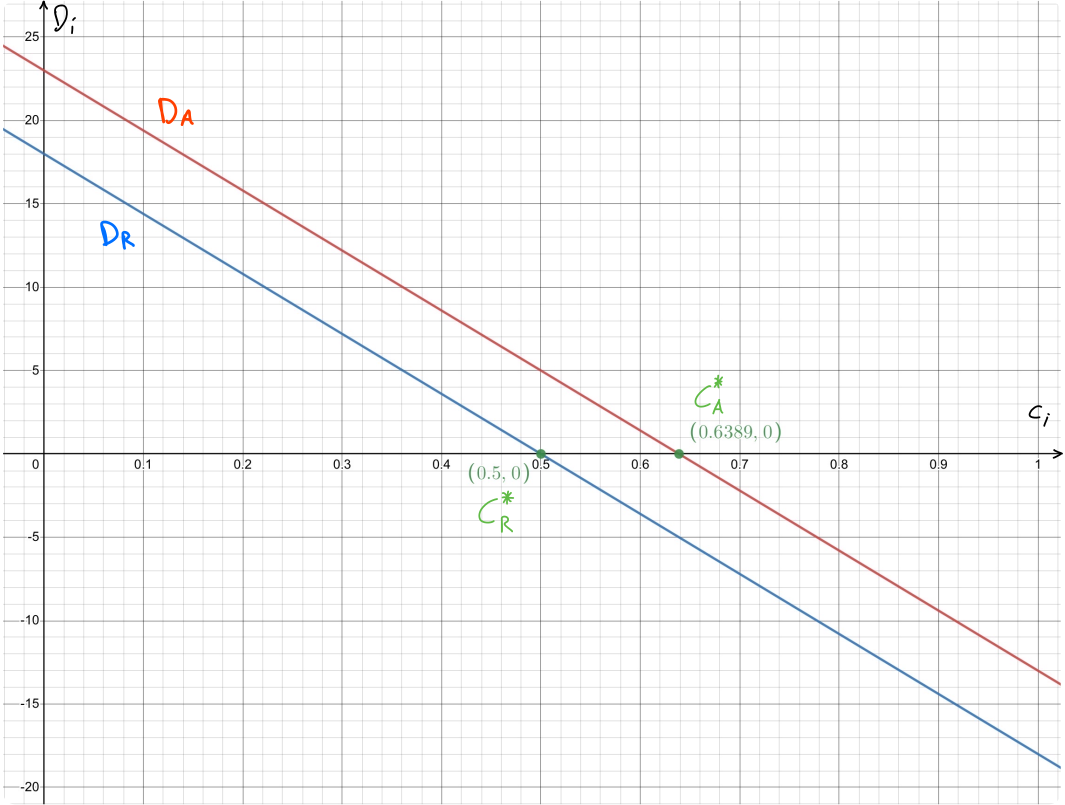
\includegraphics[width=0.8\linewidth]{figure1.png}
\caption{Decision lines for A and R as a function of $c_i$}
\label{fig:my_label}
\end{figure}


In Figure 1, we can observe how the Decision lines evolve as $c_i$ increases. When $D_i$ is positive, the player chooses to cooperate; When $D_i$ is negative, the player chooses to betray the other one. This graph also matches with reality in the CGU case, where as the investigation went on and the players felt that they were closing in on them they started getting nervous. The first to choose to betray was R and that was due to the fact that she was facing a higher possible sentence so her Decision to cooperate was more affected by the $c_R$, as her utility incorporated a higher weight on the
side of her possible sentence.

In the figure, $c_A^*$ and $c_R^*$ represent the points at which A and R will stop cooperating due to their fear of getting caught kicking in (we are assuming their $F_i = 18$ in our case), the general case would be:

\underline{$c_A^*$:}
$$
\begin{aligned}
& -5-5+F_A c_A^*(-5)-\left(-3-5-25+F_A c_A^*(-3)\right)=0 \\
& -5 F_A c_A+23+3 F_A c_A=0 \\
& 23=2 F_A c_A \rightarrow c_A^*=\frac{23}{2 F_A}
\end{aligned}
$$
\underline{$c_R^*$:}
$$
\begin{aligned}
  & -5-5+F_R c_R^*(-5)-\left(-3-5-20+F_R c_R^*(-3)\right)=0 \\ &  18=2 F_R c_R \rightarrow c_R=\frac{9}{F_R}  
\end{aligned}
$$

It becomes obvious that the point at which any of the two players will stop cooperating is whenever their combination of $F_i*c_i$ is equal to their Minimum Fear Level. We can add to the conclusion that whenever their $F_i$ is lower than the MFL, the player will always
cooperate (again, assuming that their $L_i$ = 1).


If we take into account the points at which we do not have a mathematical definition for both previous equations (i.e. whenever $F_i$ = 0 or $c_i$ = 0), we can just look at Equation 6 to conclude that in those cases, the player would just act as if they were a normal lover. This would be because if the player thinks that they are never going to get caught or if they have no fear of getting caught, they will take the common welfare into account (which leads to (C, C) being the NE), because they will be completely confident in their own welfare.
Needless to say, this situation is very theoretical.

For our sample case of $F_A = F_R = 18$:
\begin{center}
    $$c_A^* = \frac{23}{36} = 0.6389$$
    $$c_R^* = \frac{9}{18} = 0.5$$
\end{center}

Having said that, Figure 1 would only depict the relation between the decision to cooperate and $c_i$. If we want to draw the relation between $D_i$ as time passes we need to start at $c_i = f(t)$:

$$
{\left[\begin{array}{l}
c_{i 1}= a + bt \\
c_{i 2}= a \quad \Rightarrow \\
c_{i 3}= a - bt
\end{array} \text {(Meaning } c_i \text { is fixed through time)}\right.} 
$$

Therefore for each player we get 3 functions on time. Let's assume $t$ is measured in days and we simplify using the case where $a = 0$ for $c_{i1}$ and $a = 1$ for $c_{i3}$ (so $t = 0 \rightarrow c_i = 0$). Let's also assume police need 30 days to complete any investigation (i.e. $c_i = 0$ for $t = 0$ and $c_i = 1$ for $t = 30$).

We solve for $b$:

$$
\begin{aligned}
& c_{i 1}=0+b_1 t \rightarrow 1=0+b_i \cdot 30 \\
& b_1=\frac{1}{30}=0.0\overline{3} \\
& c_{i 3}=1-b_3 t \rightarrow 0=1-b_3 \cdot 30 \\
& b_3=\frac{1}{30}=b_1
\end{aligned}
$$
Thus:
$$
\begin{aligned}
& \begin{array}{l}
{\left[\begin{array}{l}
c_{i 1}=0+\frac{t}{30} \\
c_{i 2}=a_2 \quad \Rightarrow \\
c_{i 3}=1-\frac{t}{30} 
\end{array}  \text { Which implies } D_A \text { is a constant level based on } a_2 .\right.} \\ 
\vspace{5pt} \\
D_A=23-36 c_A\left\{\begin{array}{l}
D_{A 1}=23-\frac{6}{5} t \\
D_{A 2}=23-36 a_2 \\
D_{A 3}=-13+\frac{6}{5} t
\end{array}\right. \text { ($a_2$ being a stagnant probability) }
\end{array} \\
\vspace{5pt} \\
& D_R=18-36 c_R\left\{\begin{array}{l}
D_{R 1}=18-\frac{6}{5} t \\
D_{R 2}=18-36 a_2 \text { ($a_2$ being a stagnant probability) } \\
D_{R 3}=-18+\frac{6}{5} t
\end{array}\right.
\end{aligned}
$$

For the sake of simplicity we will use $a_s = 0.5$. If we graph all of the lines, we get:

\begin{figure}[htbp]
\centering
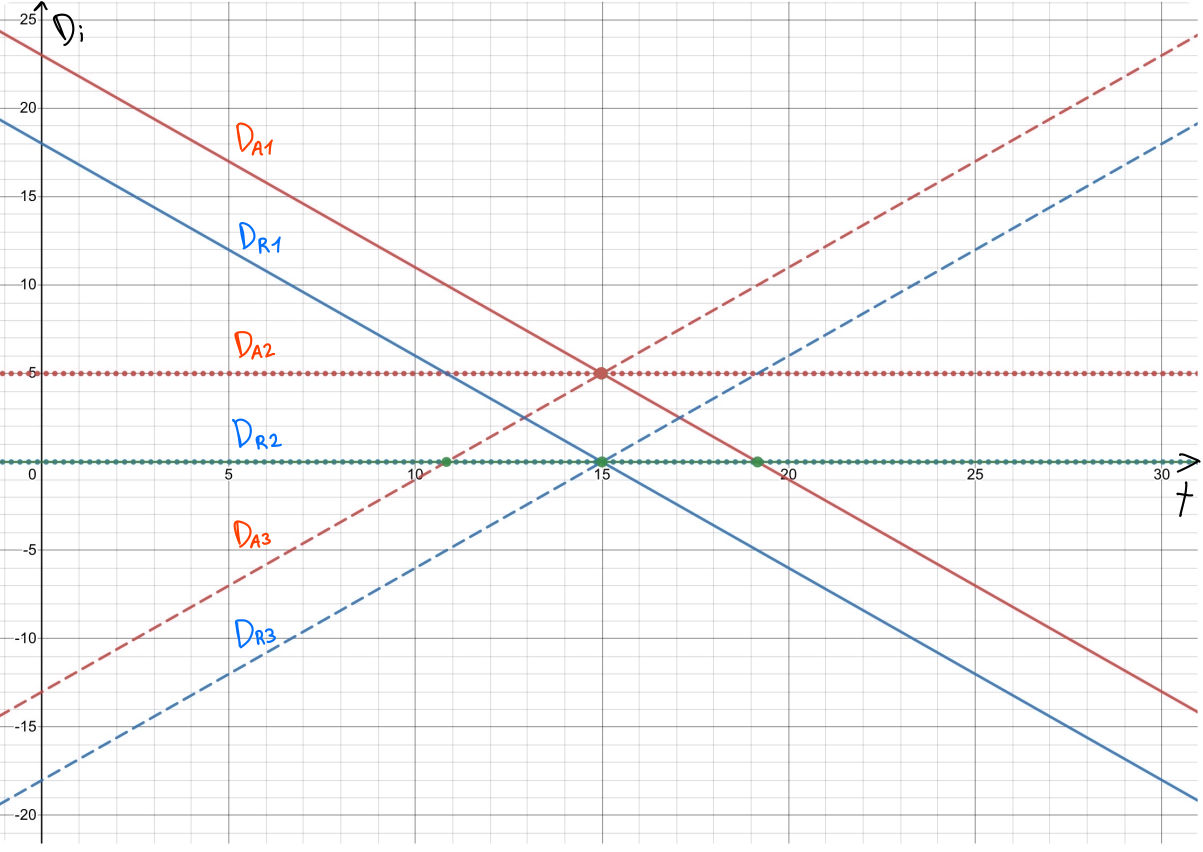
\includegraphics[width=0.8\linewidth]{figure2.png}
\caption{Decision lines studying each investigation advancement}
\label{fig:my_label}
\end{figure}

The green points highlight at what point in time every player in the CGU would change their decision on whether to cooperate or not ($D_i$). If $c_i$ increases as the investigation goes on, we can draw the conclusions presented above. In the opposite case, there would be no incentive to cooperate and both players would choose strategy B from the very beginning. On the case where the investigation becomes stagnant, it would depend at which point it happens. On the case depicted, where the investigation halts at the point $c_i$ = 0.5, we can see how A would still be willing to cooperate but R would be on the verge of betraying (again, due to her facing a higher number of years in a future
convicting sentence).

\section*{IV - Conclusions}

To conclude, let us investigate what happens when either of them chooses to betray at any given point. First we will examine how the $D_A$ would change if R decided B. At that point, let's assume she just barely passed her minimum probability ($c_R$ = 0.51) but A is still at $c_A$ = 0.5 and, thus, still cooperating.
We have a similar case as before, but instead of the decision being made by assuming the other person cooperates, now we must choose given the other person has decided to Betray:

$$
\begin{aligned}
& D_A=u\left(X_{A C} \mid B\right)-u\left(X_{A B} \mid B\right) \\
& D_A=-5-20-3+0.5 \cdot 18 \cdot(-5-20)-(-20-25+0.5 \cdot 18 \cdot(-20)) \\
& D_A=-28+9 \cdot(-25)+45+9 \cdot 20=-28
\end{aligned}
$$
$-28<0$ and therefore we can check how A would now choose B as well, as we can determine from the matrix too.

What is interesting about the CGU is that the versions that each player gave to the police, as we said above, were actually helping the police investigation against themselves. Once they chose B, they were not able to go back to output (C, C) anymore because as soon as they chose B once, $c_i$ drastically went up as well, further cementing their destiny to stay in (B, B). As a result, we can see how the state of output (C, C) is unstable and is susceptible to change as long as $F_i$ is sufficient and as long as the players are not selfless (i.e. if they are normal lovers, our basic case. In other words, if they have normal cooperation enhancing factors affecting them, for $L_i$ = 1 but also $\Omega_i$ = 1). On the other hand, though, output (B, B) is very stable and, in real life, practically inescapable.

In conclusion, for our primary case of interest (normal cooperation enhancing factors), the choice to cooperate could be treated as an iteration because players have to continue choosing to cooperate as new information is discovered by the police. In the end, though, once one of the players crosses the point of choosing B (i.e. $c_i$ > $c_i^*$), the game is closed as from there on they will always choose situation (B, B).

As a result of this, the game effectively becomes an Ultimatum Game.

To sum up, we have worked on evolving to an improved model for the Prisoner's
Dilemma which can successfully incorporate cooperation enhancing factors.
Coming from the basic PD model with the first matrix we defined, we have seen, step by step, which factors can be added in order for the model to capture the complexities we entertained.

Our goal was to study how, in reality, the situations where two prisoners have to decide whether to Cooperate or Betray the other are neither a single iteration of a PD nor an infinitely Iterated PD. Instead, PD in real life (when there are cooperation enhancing factors involved, i.e. $\Omega_i$ = 1 and $L_i$ = 1) turns into an Ultimatum Game where both players will choose C as long as $c_i$ is not too high, but at the moment $c_i$ gets higher than $c_i^*$ for any of them, they will end up in (B, B). As a result, the outcome of the game really depends on how the police investigation advances ($c_i$) and on the $F_i$ of the players (aside of the obvious $Y_{iab}$, $L_i$ and $\Omega_i$).

\nocite{*}
\printbibliography
%%%%%%%%%%%%%%%%%%%%%%%%%%%%%%%%%%%%%%%%%%%%%%%%%%%%%%%%%%%%%%%%%%
%Complete the assignment now
\end{document}

%%%%%%%%%%%%%%%%%%%%%%%%%%%%%%%%%%%%%%%%%%%%%%%%%%%%%%%%%%%%%%%%%%
%%%%%%%%%%%%%%%%%%%%%%%%%%%%%%%%%%%%%%%%%%%%%%%%%%%%%%%%%%%%%%%%%%
